% ╔══════════════════════════════════════════════════════════════╗
% ║  study-with-claude — Exam Prep LaTeX Template              ║
% ║                                                            ║
% ║  Usage:                                                    ║
% ║    1. Copy this file to your subject's exam-prep/ folder   ║
% ║    2. Replace all <PLACEHOLDERS> with your content         ║
% ║    3. Compile: pdflatex <filename>.tex                     ║
% ║                                                            ║
% ║  Or use /latex-notes to auto-generate from your materials. ║
% ╚══════════════════════════════════════════════════════════════╝

\documentclass[11pt,a4paper]{article}

% ── Layout ──────────────────────────────────────────────────────
\usepackage[margin=2cm]{geometry}

% ── Maths ───────────────────────────────────────────────────────
\usepackage{amsmath,amssymb}

% ── Lists & Tables ──────────────────────────────────────────────
\usepackage{enumitem}
\usepackage{booktabs}

% ── Headers / Sections ──────────────────────────────────────────
\usepackage{fancyhdr}
\usepackage{titlesec}

% ── Diagrams ────────────────────────────────────────────────────
\usepackage{tikz}
\usepackage[siunitx]{circuitikz}
\usetikzlibrary{arrows.meta,positioning,decorations.pathreplacing}

% ── Header / Footer ────────────────────────────────────────────
\pagestyle{fancy}
\fancyhf{}
\lhead{<MODULE-CODE> <Module Name> --- <Topic/Part>}
\rhead{<Your Name>}
\cfoot{\thepage}

% ── Section Formatting ──────────────────────────────────────────
\titleformat{\section}{\large\bfseries\itshape}{}{0em}{}
\titleformat{\subsection}{\normalsize\bfseries}{}{0em}{}
\setlength{\parindent}{0pt}
\setlength{\parskip}{4pt}

% ════════════════════════════════════════════════════════════════
\begin{document}

% ══════════════════════════════════════════════════════════════
\section*{Core Definitions}

\begin{itemize}[leftmargin=1.5em, itemsep=2pt]
  \item \textbf{<Term 1>:}
    <Definition in plain language.>
    \begin{itemize}[leftmargin=1em, itemsep=1pt]
      \item <Sub-point, example, or clarification>
      \item <Sub-point, example, or clarification>
    \end{itemize}

  \item \textbf{<Term 2>:}
    <Definition.> Use \textit{italics} for caveats or notes.
\end{itemize}

% ══════════════════════════════════════════════════════════════
\section*{Key Equations}

\textbf{<Equation name>:}
\[
  \boxed{<equation>}
\]

<Context: when to use, units, assumptions.>

\begin{itemize}[leftmargin=1.5em, itemsep=2pt]
  \item $<var>$ --- <description> (<units>)
  \item $<var>$ --- <description> (<units>)
\end{itemize}

% ══════════════════════════════════════════════════════════════
\section*{<Topic Section>}

\subsection*{<Sub-topic>}

<Prose explanation. Keep it concise --- one sentence per logical step.>

<Derivation or key result:>
\[
  \boxed{<result>}
\]

% ── Comparison Table (use when comparing methods/types) ─────
\begin{center}
\renewcommand{\arraystretch}{1.2}
\begin{tabular}{lcc}
\toprule
\textbf{Parameter} & \textbf{Type A} & \textbf{Type B} \\
\midrule
<Row 1> & <value> & <value> \\
<Row 2> & <value> & <value> \\
\bottomrule
\end{tabular}
\end{center}

% ── TikZ Block Diagram (use for system/signal flow) ─────────
\begin{center}
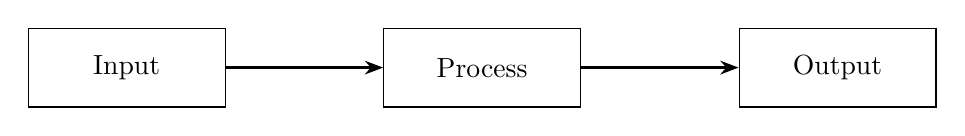
\begin{tikzpicture}[
  block/.style={draw, rectangle, minimum width=2.5cm, minimum height=1cm, align=center},
  arr/.style={->, >=Stealth, thick}
]
  \node[block] (A) {Input};
  \node[block, right=2cm of A] (B) {Process};
  \node[block, right=2cm of B] (C) {Output};
  \draw[arr] (A) -- (B);
  \draw[arr] (B) -- (C);
\end{tikzpicture}
\end{center}

% ── Circuit Diagram (use for electrical circuits) ────────────
\begin{center}
\begin{circuitikz}[scale=1.0, every node/.style={font=\small}]
  \draw (0,0) to[V, l=$V_S$] (0,3)
              to[R, l=$R_1$] (3,3)
              to[R, l=$R_2$] (3,0) -- (0,0);
\end{circuitikz}
\end{center}

% ══════════════════════════════════════════════════════════════
\section*{Worked Examples}

\subsection*{Example 1: <Short description>}

\textbf{Given:} $<param_1> = <value>$, $<param_2> = <value>$.

\textbf{Find:} <What to calculate.>

\textbf{Solution:}
\[
  <working> = \mathbf{<answer with units>}
\]

\subsection*{Example 2: <Multi-part>}

\begin{enumerate}[leftmargin=1.5em, itemsep=2pt]
  \item[(i)] \textbf{<Part description>:}
    <Working> $= \mathbf{<answer>}$.

  \item[(ii)] \textbf{<Part description>:}
    <Working> $= \mathbf{<answer>}$.
\end{enumerate}

% ══════════════════════════════════════════════════════════════
\section*{Summary}

\begin{itemize}[leftmargin=1.5em, itemsep=2pt]
  \item <Key takeaway 1 --- include the core equation or fact>
  \item <Key takeaway 2 --- note any common pitfalls>
  \item <Key takeaway 3 --- link to related topics>
\end{itemize}

% ══════════════════════════════════════════════════════════════
\section*{Checklist}

\begin{itemize}[leftmargin=1.5em, itemsep=1pt]
  \item[$\square$] Can you define all core terms from this topic?
  \item[$\square$] Can you derive the key equations from first principles?
  \item[$\square$] Can you \textbf{draw} the relevant diagrams/circuits from memory?
  \item[$\square$] Can you solve the worked examples without looking at the solution?
  \item[$\square$] Can you explain the physical intuition behind each equation?
\end{itemize}

\end{document}
